\chapter{Implementation}
% This chapter should describe what was actually produced: the programs which were written, the hardware which was built or the theory which was developed. Any design strategies that looked ahead to the testing stage might profitably be referred to (the professional approach again).
% Descriptions of programs may include fragments of high-level code but large chunks of code are usually best left to appendices or omitted altogether. Analogous advice applies to circuit diagrams.
% Draw attention to the parts of the work which are not your own. The Implementation Chapter should include a section labelled ”Repository Overview”. The repository overview should be around one page in length and should describe the high-level structure of the source code found in your source code Repository. It should describe whether the code was written from scratch or if it built on an existing project or tutorial. Making effective use of powerful tools and pre-existing code is often laudable, and will count to your credit if properly reported.
% It should not be necessary to give a day-by-day account of the progress of the work but major milestones may sometimes be highlighted with advantage.

%  ~4,500 words

% Tangent works better than correlation or partial correlation.
\section{Overview}

\begin{figure}[]
    \centering
    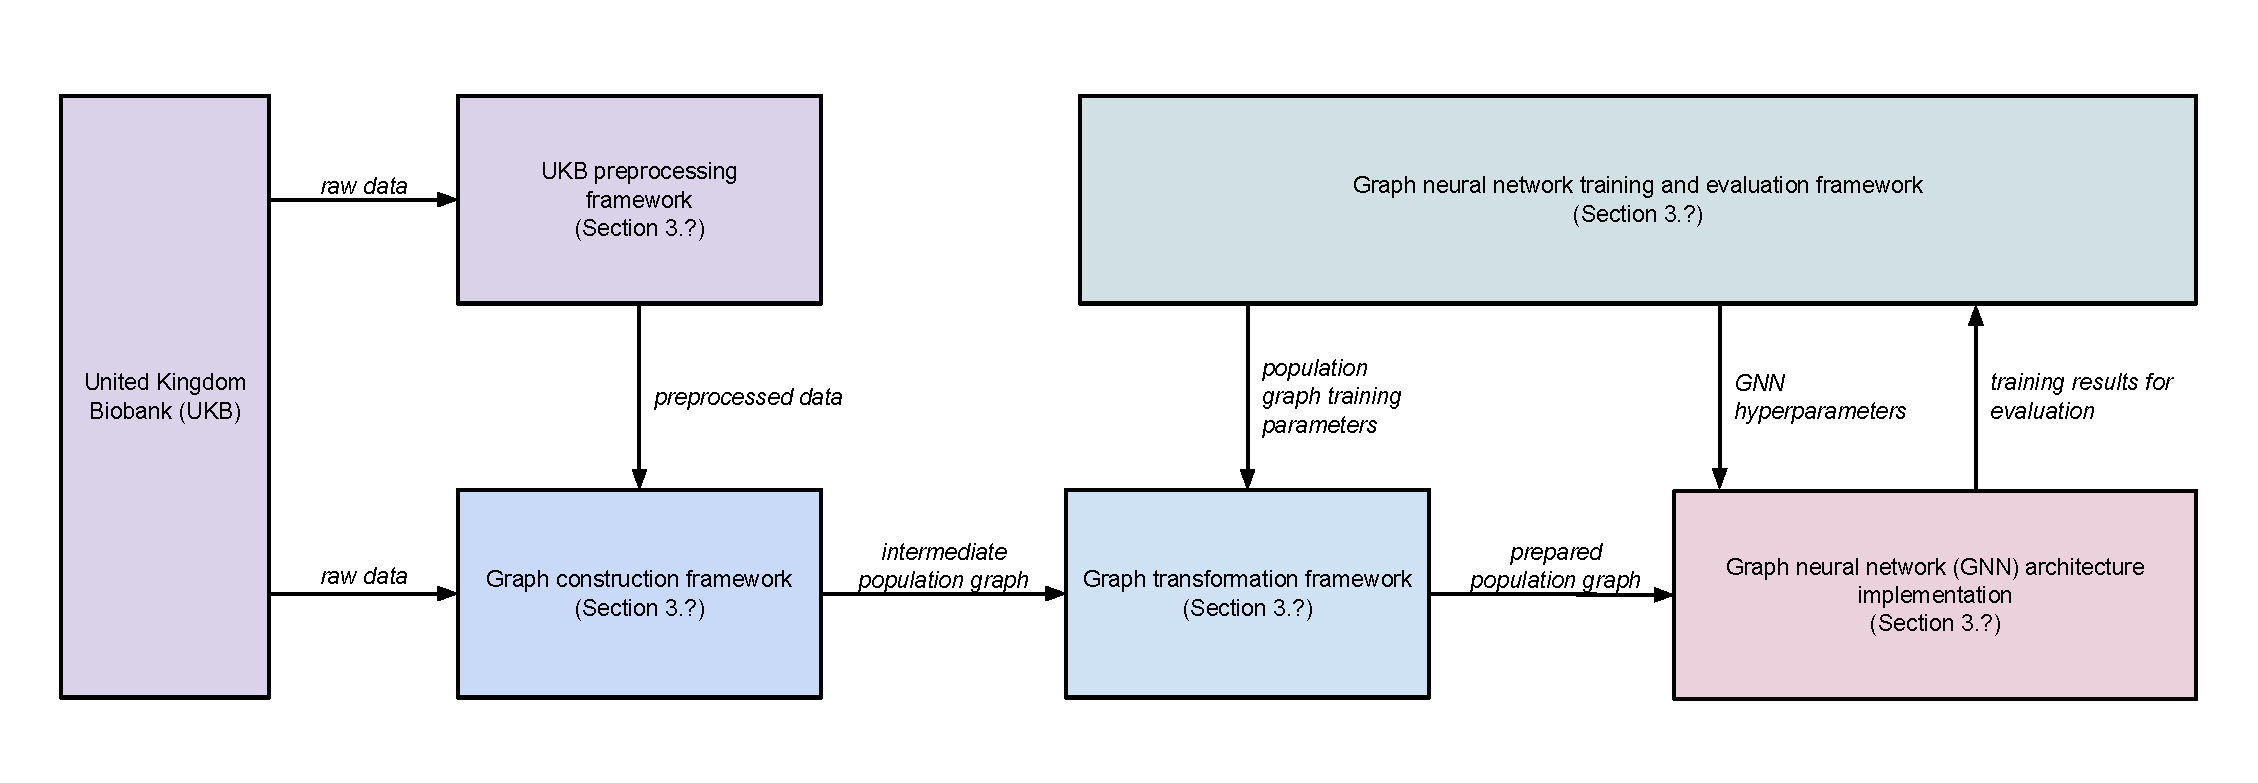
\includegraphics[width=\textwidth]{pipeline_overview.pdf}
    \caption{Overview of the key project components.}\label{pipeline-overview}
\end{figure}

This project can be divided into five key components (Figure~\ref{pipeline-overview}):
\begin{enumerate}
    \item Preparation of the United Kingdom Biobank (UKB) dataset;
    \item Intermediate population graph construction;
    \item Population graph transformation for training;
    \item Training on graph neural network architectures;
    \item Evaluation of the graph neural network performance.
\end{enumerate}

This chapter will explain in detail the steps behind each of the stages.

TODO fill the page (can make a bigger diagram!)


\section{UKB preprocessing component}

\begin{figure}[!htb]
    \centering
    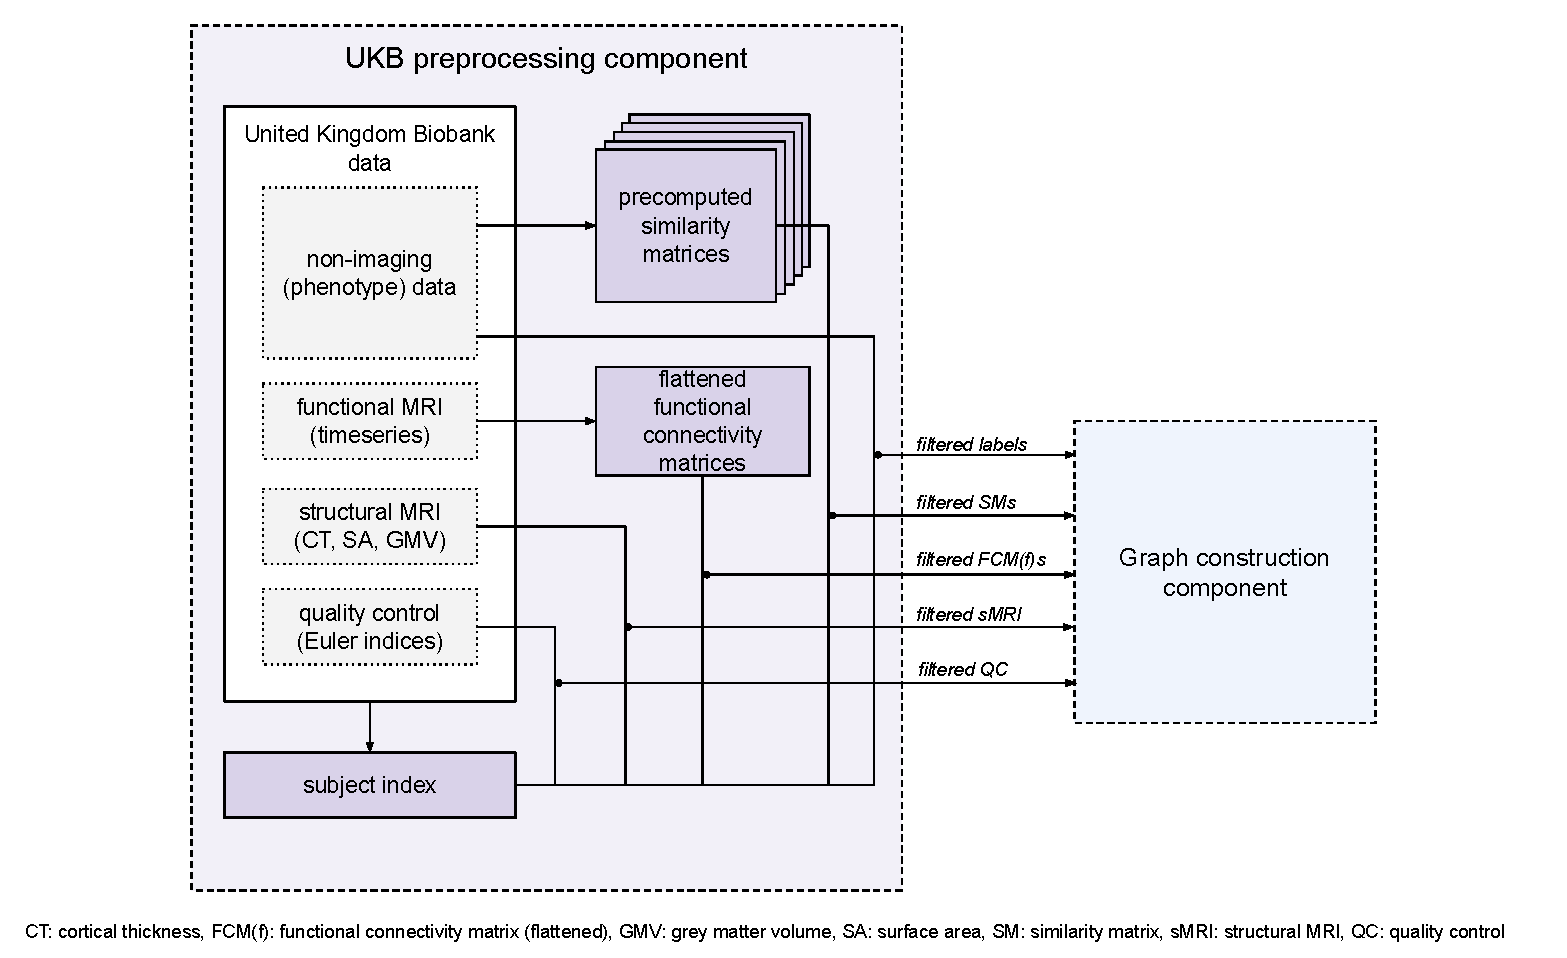
\includegraphics[width=\textwidth]{preprocessing_component.pdf}
    \caption{UKB preprocessing component.}\label{preprocessing-component}
\end{figure}

The main function of the UKB preprocessing component is to prepare the raw or partially preprocessed UKB data for population graph construction (Figure~\ref{preprocessing-component}). In particular, to improve the computational efficiency of most of the operations later in the pipeline, this component precomputes some of the data in the convenient form. This involves cleaning the dataset, precomputing similarity matrices and functional connectivity matrices.

\subsection{Cleaning the dataset}
While the United Kingdom Biobank is very well maintained and the data is nicely structured, the different modalities (functional MRI, structural MRI, phenotype data, Euler indices—as shown by different components in Figure~\ref{preprocessing-component}) were provided separately. The functional data contains scans for 17,550 patients, but 233 of them had missing data in other modalities (it was retracted from the Biobank but the scans remained available). Three more patients have had corrupted brain scans (did not have a matching number of brain regions), which resulted in functional connectivity matrices being different from all the others (and consequently a different number of features) and were therefore discarded. The 17314 patients that had the data available for all modalities have been collected into a subject index. The data from all modalities are filtered using this subject index before being selected for population graph construction.

\subsection{Precomputing connectivity matrices}
The connectivity matrices involve computing the pairwise correlations of 376 time-series for every subject, a $O(N^2)$ computation for the dataset of  $N$ subjects. With 20 GB of raw timeseries data across over 17,000 subjects, this introduces a high computational overhead (a few hours) if the matrices are computed on the fly as the graph is constructed. An additional inefficiency comes from the computation being repeated whenever a population graph that uses the functional data is constructed (which might be frequent when different graph parameterisations are explored). To avoid the inefficiency, the matrices are computed once for each subject, flattened and their lower triangles stored as NumPy arrays as part of the preprocessing component.

TODO could include the maths here?

\subsection{Precomputing similarity matrices}
While the non-imaging modalities used for similarity computation are much smaller in file size, the computation of the similarity function is also pairwise. The $O(N^2)$ computation that involves pairwise comparison, addition and averaging of values for each non-imaging metric might take hours or even days for the full dataset to be processed, depending on the exact similarity definition. This computation is also repeated whenever a graph is constructed, since the similarities per non-imaging metric do not change over different graphs: the variation comes from different selections of metrics, their relative weighting, and similarity thresholds.

The similarity matrices for the non-imaging features in Table~\ref{table:phenotype-features} have therefore been computed in advance. Unlike the functional connectivity data used directly as node features, the metric-wise similarities need to be looked up quickly when computing the score for a given similarity function, so the full matrix is stored.


For the \texttt{ICD10} metric, the subjects were considered to be \texttt{ICD10}-similar whenever they had at least one shared mental health or nervous system diagnosis, while two patients without any mental health or nervous system diagnoses were \textit{not} considered to be similar, as this would create too many edges and make the model run out of memory. The computation can be vectorised: for the boolean \texttt{ICD10}-lookup matrix $\mathbf{F}_{\text{icd10}}$ with rows indexed by subjects and columns by relevant \texttt{ICD10} diagnoses, the pairwise similarity matrix $\mathbf{M}_{\text{icd10}}$ computation corresponds to 

\begin{equation}
    \mathbf{M}_{\text{icd10}} = \mathbf{1}\left[\mathbf{F}_{\text{icd10}}^{\ }\mathbf{F}_{\text{icd10}}^{\mathrm{T}} \geq 1\right]
\end{equation}

where the indicator function $\mathbf{1}[\cdot]$ is applied element-wise.

For the remaining metrics (e.g. years of full-time education, \texttt{FTE}) there is only one integer or floating-point value per subject, with values  compared for equality. The operation is vectorised by exploiting NumPy's broadcasting operation that copies rows and columns as necessary for the matrix dimensions to match: for the vector of subject \texttt{FTE}s $\mathbf{f}_{\text{fte}}^{\mathrm{T}} \in \mathbb{R}^{N \times 1}$ and $\mathbf{F}_{\text{fte}} = [\mathbf{f}_{\text{fte}}^{\mathrm{T}} \cdots \mathbf{f}_{\text{fte}}^{\mathrm{T}}] \in \mathbb{R}^{N \times N}$, \texttt{FTE}-similarity matrix is defined as

\begin{equation}
    \mathbf{M}_{\text{fte}} = \mathbf{1}\left[\mathbf{F}_{\text{fte}}^{\ } = \mathbf{F}_{\text{fte}}^{\mathrm{T}} \right].
\end{equation}


% \[
% \begin{blockarray}{rccccc}
%  & b & c & d & e & f \\
% \begin{block}{r[ccccc]}
%   \text{UKB} & 1 & 1 & 1 & 1 & f \\
%   0 & 1 & 0 & 0 & 1 & g \\
%   0 & 0 & 1 & 0 & 1 & h \\
%   0 & 0 & 0 & 1 & 1 & i \\
%   0 & 0 & 0 & 0 & 1 & j \\
% \end{block}
% \end{blockarray}
%  \]


\section{Graph construction component}

\begin{figure}[h]
    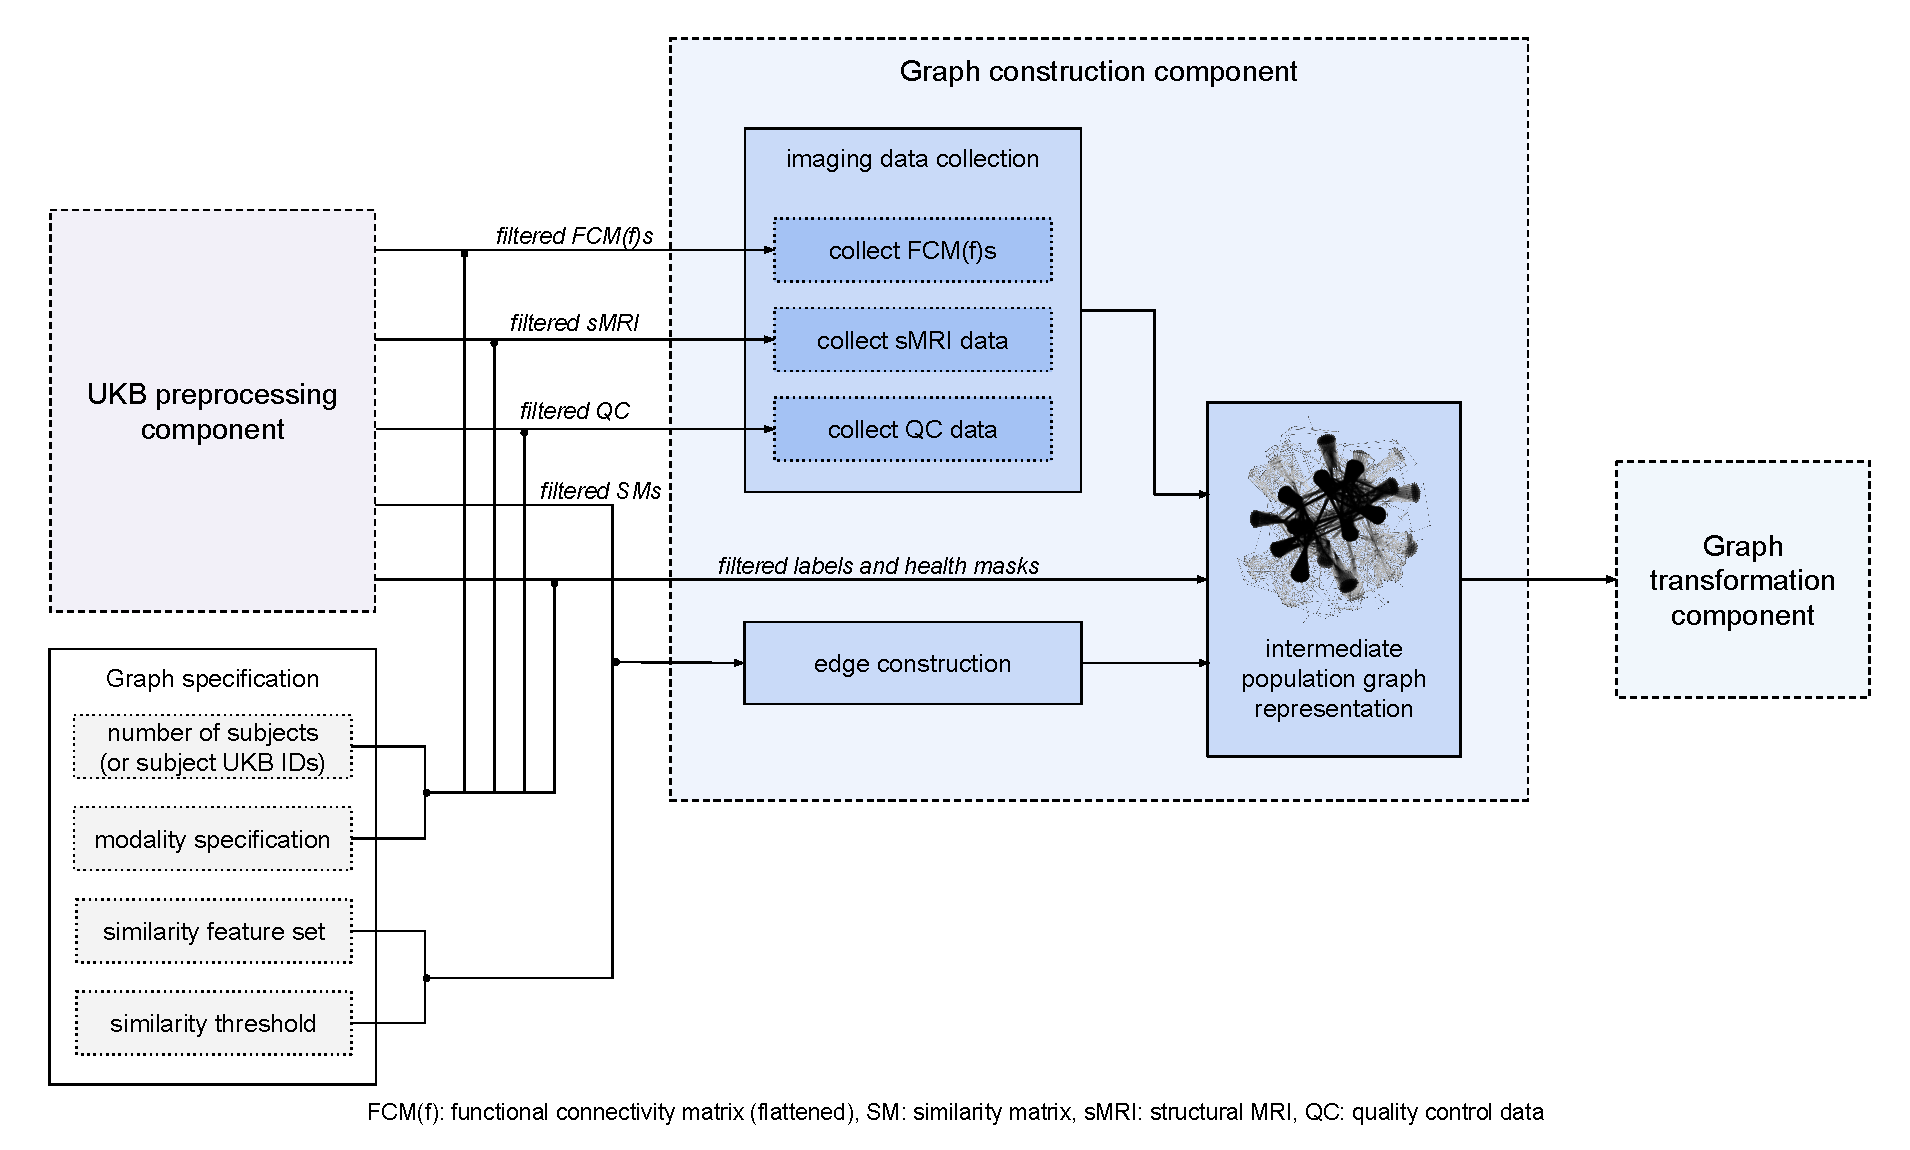
\includegraphics[width=\textwidth]{graph_construction_component.pdf}
    \caption{Graph construction component.}\label{graph-construction-component}
\end{figure}

The next stage of the pipeline involves constructing the ``intermediate representation'' of the population graph, which contains the graph topology and node features but is not prepared for training (is not split into training, validation and test sets, and the features are not normalised). The two stages are separate because the same intermediate representation can be reused many times for different dataset split and other evaluation parameters without having to reconstruct the topology in $O(N^2)$ time. The steps for how the data is processed in this component is schematically visualised in Figure~\ref{graph-construction-component}.

\subsection{Inputs}
The inputs to the graph construction component can be categorised into four main types as shown in the white box at the bottom left of Figure~\ref{graph-construction-component}. These are subject specification, modality specification, similarity feature set and similarity threshold parameters.

\textit{Subject specification} takes in the number of (randomly selected) subjects that should be used in creating the graph, or UKB identifiers for the list of specific subjects. If no parameter is provided, then all available data is used for population graph construction.

\textit{Modality specification} describes which of the neuroimaging modalities should be used as node features, which could be a combination of functional, structural and quality control data.

\textit{Similarity feature set}. 
TODO maybe rename similarity specification (because it can either be a feature set or function)

In its default implementation, the similarity metric is computed as the average score across a set of similarity features $\{M_1, \dots, M_n\}$ (see Equation~\eqref{eq:similarity}). 

TODO extension: arbitrary similarity functions.

\textit{Similarity threshold}. A number $\mu \in [0,1]$ defining the threshold for the similarity metric above which an edge will be added to the graph (see Equation~\eqref{eq:similarity-threshold}).

\subsection{Imaging data collection}

Based on the number of subjects and modalities provided, the relevant imaging data is collected from the raw UKB files (first filtered by subject index as discussed before) and stored in the intermediate representation in its original form as a dataframe indexed by subject. If the modality is unused, an empty dataframe is stored.


\subsection{Edge construction}

This component uses the subject set and the similarity specification provided to combine the individual similarity metrics into an overall similarity score for each pair of subjects, then comparing it to the similarity threshold and adding an edge if the score exceeds the threshold.

\subsection{Brain health mask computation}

Due to the nature of the brain age problem, the population graph can only be trained on subjects with healthy brains, although it may contain both healthy and non-healthy subjects. The \textit{brain health mask} is computed to determine which subjects can be included in training and which cannot. In this project, the brain health is approximated by the absence of diagnoses related to mental health or nervous system disorders, defined by the \texttt{ICD10} metric (see Table~\ref{table:phenotype-features}).

\subsection{Population graph representation}

\renewcommand{\arraystretch}{1.25}
% \begin{table}[]
%     \caption{The population graph data structure (excludes helper or utility fields).}\label{table:population-graph}
%     \centering
%     \begin{tabular}{lp{0.2\textwidth}p{0.5\textwidth}}
%         \hline
\begin{center}
\begin{longtable}{lp{0.175\textwidth}p{0.475\textwidth}}
    \caption{The population graph data structure.}\label{table:population-graph}\\
    \hline \textbf{Field name} & \textbf{Type} & \textbf{Description} \\
    \hline
    \endfirsthead
    \multicolumn{3}{c}%
    {\tablename\ \thetable\ -- \textit{Continued from previous page}} \\
    \hline
    \textbf{Field name} & \textbf{Type} & \textbf{Description} \\
    \hline
    \endhead
    \hline \multicolumn{3}{r}{\textit{Continued on next page}} \\
    \endfoot
    \hline
    \endlastfoot
    
    \texttt{num\_nodes} & long & Number of nodes (subjects) in the population graph. \\
    \texttt{subject\_index} & string vector & UKB identifiers of the subjects. Stored in the order of mask, feature and label vector indices; corresponds to the edge start and end values. \\
    \texttt{brain\_health\_mask} & boolean vector & \texttt{True} indicates that the subject can be used for training, and \texttt{False} otherwise. \\
    \texttt{edge\_index} & $2\times 2|E|$ \hfill\newline long tensor & \texttt{edge\_index}$[0][i]=s_v$ and \hfill \newline \texttt{edge\_index}$[1][i]=s_w$ indicate a directed \hfill \newline edge $s_v \leadsto s_w$. To represent the undirected edge $(s_v, s_w) \in E$, the second directed edge $s_w \leadsto s_v$ is added. \\
    \texttt{y} & $N \times 1$ \hfill \newline float tensor & Contains the labels of training data, in this case chronological age. \\
    \texttt{functional\_data} & dataframe & Row-indexed by subject with columns containing the flattened functional connectivity matrix entries. Empty if no functional data is used in the population graph. \\
    \texttt{structural\_data} & dictionary of \hfill \newline dataframes & Dictionary is indexed by the structural data modality, in this case cortical thickness, surface area, and grey matter volume. The corresponding dataframes are row-indexed by subject with columns containing the features of the relevant structural data modality. The dataframes are empty if no structural data is used. \\
    \texttt{quality\_control\_data} & dataframe & Row-indexed by subject with the columns containing Euler indices for the left and right hemispheres of the brain. Empty if no quality control data is used. \\
    \texttt{name} & string & The name of the population graph. \\
    \texttt{X} & $N \times F$ \hfill\newline float tensor & \textit{Unused at the intermediate stage.} Contains the full normalised feature vector (of $F$ features) for every graph node (subject). \\
    \texttt{train\_mask} & boolean tensor & \textit{Unused at the intermediate stage.} \texttt{True} if the subject belongs to the training set, and \texttt{False} otherwise. \\
    \texttt{validation\_mask} & boolean tensor & \textit{Unused at the intermediate stage.} \texttt{True} if the subject belongs to the validation set, and \texttt{False} otherwise. \\
    \texttt{test\_mask} & boolean tensor & \textit{Unused at the intermediate stage.} \texttt{True} if the subject belongs to the test set, and \texttt{False} otherwise.
    % \end{tabular}
\end{longtable}
\end{center}

The population graph is extended from the base Pytorch Geometric \texttt{Data} object, with its main fields listed in Table~\ref{table:population-graph}. The intermediate version has all entries defined except the feature vector \texttt{X} and the training, validation and test masks.

TODO ordering of members based on their use order in the pipeline, meaning (training vs data etc.)

TODO Could here mention the \textit{extension} of having weighted edges where edge features would store raw similarities as long as they exceed the threshold (to avoid $O(N^2)$ entries).


\section{Graph transformation component}

\begin{figure}[h]
    \centering
    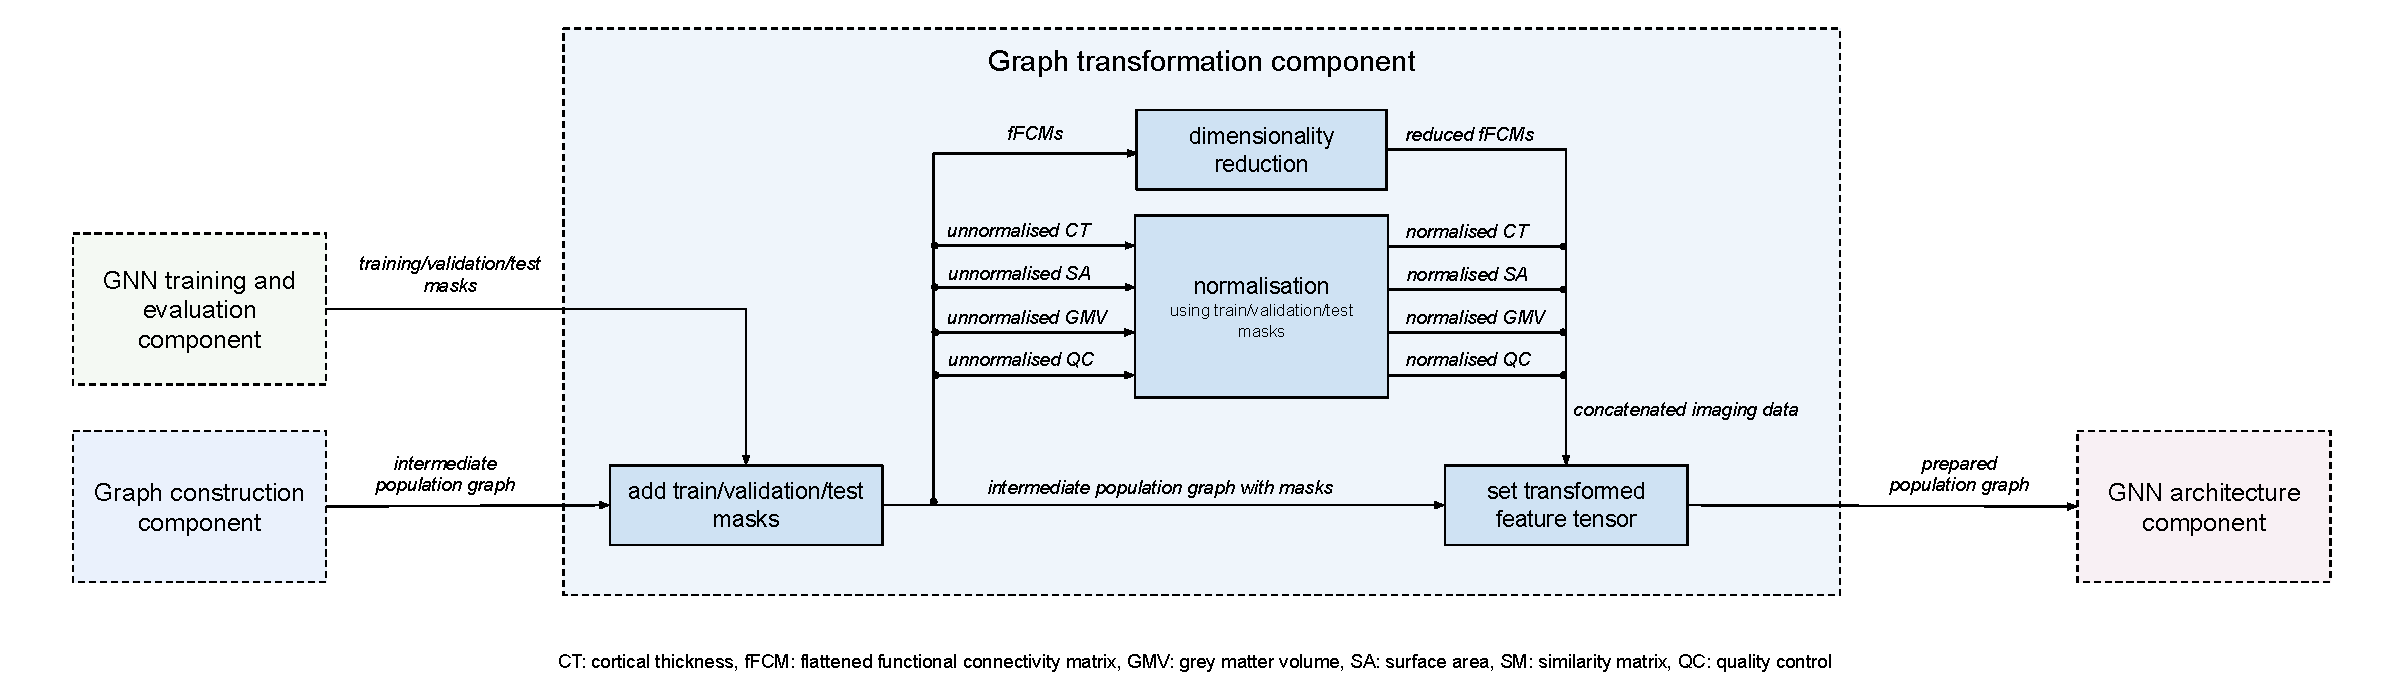
\includegraphics[width=\textwidth]{graph_transformation_component.pdf}
    \caption{Graph transformation component.}\label{graph-transformation-component}
\end{figure}

The graph transformation component is responsible for preparing the intermediate population graph representation for training by defining its normalised and combined feature vector as well as training, validation and test masks. The schematic diagram representing the steps in this component is shown in Figure~\ref{graph-transformation-component}.

Describe how the graph intermediate representation is changed based on the training transformation parameters (training fold, train/validation/test set split). The intermediate graph is prepared for training by normalising the features based on the train subset, adding train/validation/test set masks to ignore subjects that should not be used for feedback in training, concatenating the multiple modalities into a single feature set.

Subject stratification, removing subjects with too few age occurrences because the data cannot be correctly stratified otherwise.


\section{Graph neural network component}
Description of architecture: number and size of layers etc.

Could have a diagram.


\section{Evaluation component}
The standard performance metrics $r$ and $r^2$ tracked and logged with training.

Describe the additional graph transformation stages which add noise to node features/edges.


\section{Repository overview}
% The repository overview should be around one page in length and should describe the high-level structure of the source code found in your source code Repository; ... could be implemented as a table with folders/file names and the functionality implemented in those files


\newpage




\subsection{Functional connectivity matrix precomputation}

\subsubsection{Dimensionality reduction for neural networks}
The full flattened functional connectivity matrix has over 75,000 features per patient, which, considering pairwise similarities and a large number of subjects, makes the graph (and the training on it) very large: the number of resulting training parameters runs out of memory even for small architectures.

The easiest solution mitigating this is running a PCA on the matrix, assuming that the first few principal components (how many?) would give a good representation of functional data features. Preliminary runs on small datasets of a few thousand subjects give similar performance.



\subsection{Hyperparameter tuning}
Describe which hyperparameters were tuned using Bayesian optimisation strategy, early stopping, cross-validation etc.




